%UNIT 1: QUALITATIVE AND GRAPHICAL APPROACHES
% Is first part of original 01.tex
%%%%%%%%%%%%%%%%%%%%%%%%%%%
%%%% Put the following at the top of each .tex file  %
\pagestyle{fancy}
\renewcommand{\theUnit}{2}
\ifthenelse{\isundefined{\UnitPageNumbers}}{}{\setcounter{page}{1}}
\rhead{Carlton and Devore Chapter \theUnit: Discrete Random Variables}
\lhead{Math 3382: Statistical Theory}
%\lhead{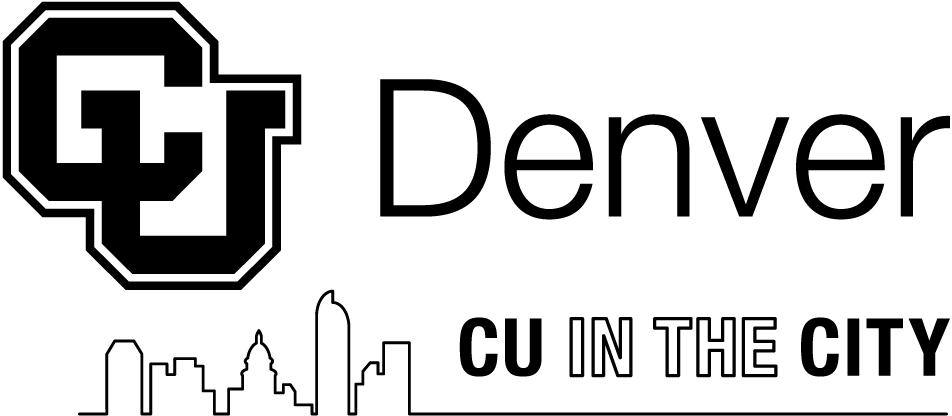
\includegraphics[width=1.25cm]{CUDenver-Logo.png}}
\rfoot{\mypage}
\cfoot{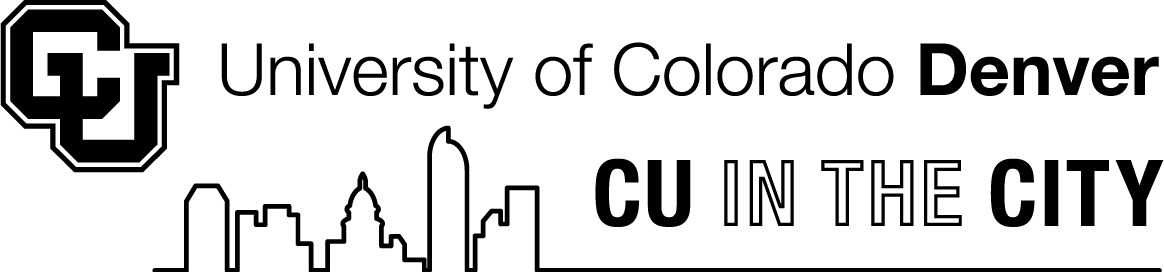
\includegraphics[width=2.25cm]{CUDenver-Logo-coverpage.png}}
\lfoot{Adam Spiegler}
\fancypagestyle{firstfooter}{\footskip = 50pt}
\renewcommand{\footrulewidth}{.4pt}
%%%%%%%%%%%%%%%%%%%%%%%%%%%
\vspace*{-20pt} \thispagestyle{firstfooter}

\pagebegin{Discrete Random Variables}

\bb
\ii Suppose a company knows that 1\% of the lithium batteries they manufacture are defective.  The manufacturer sends a shipment of 10 batteries to one of their clients. Let the random variable $X$ denote the number of good (not defective) batteries in the shipment. How likely is it that exactly two of the batteries are defective? \label{q:batteries}

\bb
\ii What is the probability of getting the outcome $GGGGGGGGDD$? Note $G$ and $D$ denote good and defective batteries, respectively. \vfill
\ii How many outcomes are in the event exactly 2 out of 10 batteries are defective? \vfill
\ii Calculate $P(X=8)$. \vfill
\ee

\ii Generalize the result in the previous example. If you repeat $n$ trials which are independent from one another, and each has the same probability of success, $p$, what is the probability of getting exactly $s$ successes out of $n$ trials? \bigskip

$\dsty f(s) = P(X=s) =$   \bigskip

\ii How many good batteries would you expect to receive if you had a shipment of 100 batteries (where it is known that $1$\% of all batteries are defective)? If you received a shipment of 200 batteries? A shipment of 10 batteries? \vfill

\ii Write a general formula for the expected number of successes when $n$ trials are repeated with probability of success $p$ in each trial. \vfill

\ee

\clearpage

\pagebegin{Binomial Distributions}

\begin{tcolorbox}
\bi
\ii A \textbf{\colorb{Bernoulli trial}} is an experiment that has \textbf{\colorb{exactly two possible outcomes}}:
\bi
\ii[$\circ$] The probability that the outcome of a trial is a \colorb{success} ($X=1$ ) is denoted \colorb{$p$}.
\ii[$\circ$] Otherwise, the probability of a \colorr{failure} ($X=0$ ) is \colorr{$q=1-p$}.
\ii[$\circ$] $X$ has a \textbf{\colorb{Bernoulli Distribution}} with probability mass function
\[ f(x) = p^x(1-p)^{1-x} \ \ , \mbox{for } x \in \left\{ 0, 1 \right\}.\]
\ei

\ii Let random variable $X$ be the number of successes out of $n$ trials, where \colorb{each trial is identical and independent}. 
\bi
\ii[$\circ$] $X$ has a \textbf{\colorb{Binomial Distribution}}, written $X \sim \mbox{Binomial}(n,p)$.
\ii[$\circ$] The probability mass function is
\[ f(x) = \left\{ \begin{array}{ll} \left( \begin{array}{c} n\\ x \end{array} \right) p^x(1-p)^{n-x} \ \ & \mbox{for } x =0,1,2, \ldots , n\\
 & \\
0 \ \ & \mbox{otherwise} \end{array} \right. .\]
\ii[$\circ$] The expected value can be calculated with the shortcut \colorb{$E(X) = np$}.
\ii[$\circ$] The variance can be calculated with the shortcut \colorb{$\Var(X) = npq$}.
\ei
\ei
\ebox

\medskip

\begin{tcolorbox}
In R, the we can use the functions:
\bi
\ii \colorb{dbinom($x$, $n$, $p$)} calculates the probability of \colorb{exactly $x$ success} out $n$ trials, \colorb{$P(X=x)$}. 
\ii \colorr{pbinom($x$, $n$, $p$)} calculates the probability of \colorr{at most $x$ success} out $n$ trials, \colorr{$P(X \leq x)$}. 
\ei
\end{tcolorbox}

\bb[resume]
\ii Consider the lithium battery example from question \ref{q:batteries}. Write a command in R that computes the given probability.
\bb
\ii Exactly 7 batteries are good. \vfill
\ii At most 8 batteries are good. \vfill
\ii At most 4 batteries are defective. \vfill
\ee
\ee

\clearpage

\pagebegin{Equally Likely Outcomes}

\bb[resume]
\ii Let $X$ be the value of the result of rolling a fair six-sided die.
\bb
\ii Write out the probability mass function $f(x)$. \vfill
\ii What is the expected value of rolling a fair-six sided die? \vfill
\ee
\ee


\bbox
Let $X$ be a discrete random variable with $k$ different outcomes that each have the same likelihood of occurring.
\bi
\ii $X$ has a \textbf{\colorb{uniform distribution}} on $\left\{ 1, 2, 3, \ldots , k \right\}$
\ii The probability mass function is 
\[ f(x) = \left\{ \begin{array}{ll} \frac{1}{k} \ \ & \mbox{for } x = 1, 2, \ldots,  k\\
0 \ \ & \mbox{otherwise} \end{array} \right. .\]
\ii The expected value is $E(X) = \frac{k+1}{2}$.
\ii The variance is $\Var(X) = \frac{k^2-1}{12}$.
\ei 
\ebox

\bb[resume]
\ii A sports marketer for the Denver Nuggets randomly calls people in the Denver area until she encounters someone who attended a Nuggets' game. What is the probability the market encounters $7$ people who did not attend a game before the first success when it is known that 10\% of the population attended a game last season? \vfill
\ee

\clearpage

\pagebegin{Number of Failures Before First Success}


\bbox
If we repeat a Bernoulli trial that has probability of success $p$ for each trial, we can \colorb{count the number of failures, $X$, that occur before the first success.}
\bi
\ii $X$ has a \textbf{\colorb{Geometric Distribution}}, written $X \sim \mbox{Geom}(p)$.
\ii The probability mass function is $\dsty f(x) = q^xp$ for $x \in \lbrace 0, 1, \ldots \rbrace$.
\ii The expected value is $\mu=E(X) = \frac{q}{p}$.
\ii The variance is $\sigma^2 = \Var(X) = \frac{q}{p^2}$.
\ei

\medskip

In R, the we can use the functions:
\bi
\ii \colorb{dgeom($x$, $p$)} calculates the probability of \colorb{exactly $x$ failures} before first success. 
\ii \colorr{pgeom($x$, $p$)} calculates the probability of \colorr{at most $x$ failures} before first success.
\ii There is no fixed number of trials $n$.
\ei 
\ebox

\pagebegin{Number of Occurrences in a Fixed Time Period}

\bbox
The \textbf{\colorb{Poisson distribution}} applies when the average frequency of occurrences in a given time period is known, and each occurrence is independent the others. Let $X$ denote \colorb{the number of occurrences in the given time period}.
\bi
\ii $X \sim \mbox{Poisson}(\lambda)$, where $\lambda$ denotes the mean number of occurrences in the given time.
\ii The probability mass function is $\dsty f(x) = e^{-\lambda} \frac{\lambda^x}{x!}$ for $x \in \lbrace 0, 1, 2, \ldots \rbrace$.
\ii The expected value is $\mu = E(X) = \lambda$.
\ii The variance is $\sigma^2 = \Var(X) = \lambda$ (same as the expected value).
\ei 

\medskip

In R, the we can use the functions:
\bi
\ii \colorb{dpois($x$, $\lambda$)} calculates the probability of \colorb{exactly $x$ occurrences} in the given time.
\ii \colorr{ppois($x$, $\lambda$)} calculates the probability of \colorr{at most $x$ occurrences} in the given time.
\ei %\bigskip
\ebox

\bb[resume]
\ii If there are twelve cars crossing a bridge per minute on average, find the probability of having seventeen or more cars crossing the bridge in a particular minute.
\ee

\vfill

\clearpage

\pagebegin{Practice}

\bb[resume]
\ii For each situation, identify which distribution best describes the distribution of the random variable. Then use a probability distribution function to calculate the probability.
\bb
\ii A online retailer sells an average of 5 big screen TV's on a given day. What is the probability they sell 9 TV's in a day? \vfill
\ii It is known that 3\% of airbags manufactured by a certain car company are defective. What is the probability that the first defective air bag occurs when the fifth item is inspected? \vfill
\ii Recently, a nurse commented that when a patient calls the medical advice line claiming to have the flu, the chance that he or she truly has the flu (and not just a nasty cold) is only about 4\%. Of the next 25 patients calling in claiming to have the flu, what is the probability that exactly 4 patients will have the flu? \vfill
\ee
\ee
